\chapter{Prototipado del algoritmo en software}

\section{Flujo del algoritmo}
Como se ha explicado anteriormente, el algoritmo realizará una recopilación de datos para obtener la señal original del electrocardiograma de cada paciente y así hacer un filtrado de dicha señal para eliminar el ruido y centrarla, seguidamente se realizará la detección de picos con algunos métodos como establecer el \textit{cutoff} dinámico y por último detectar las arritmias y comparar las anotaciones de la señal original con las generadas. Véase \Cref{fig:esquemaGeneral}.

\begin{figure}[h!]
    \centering
    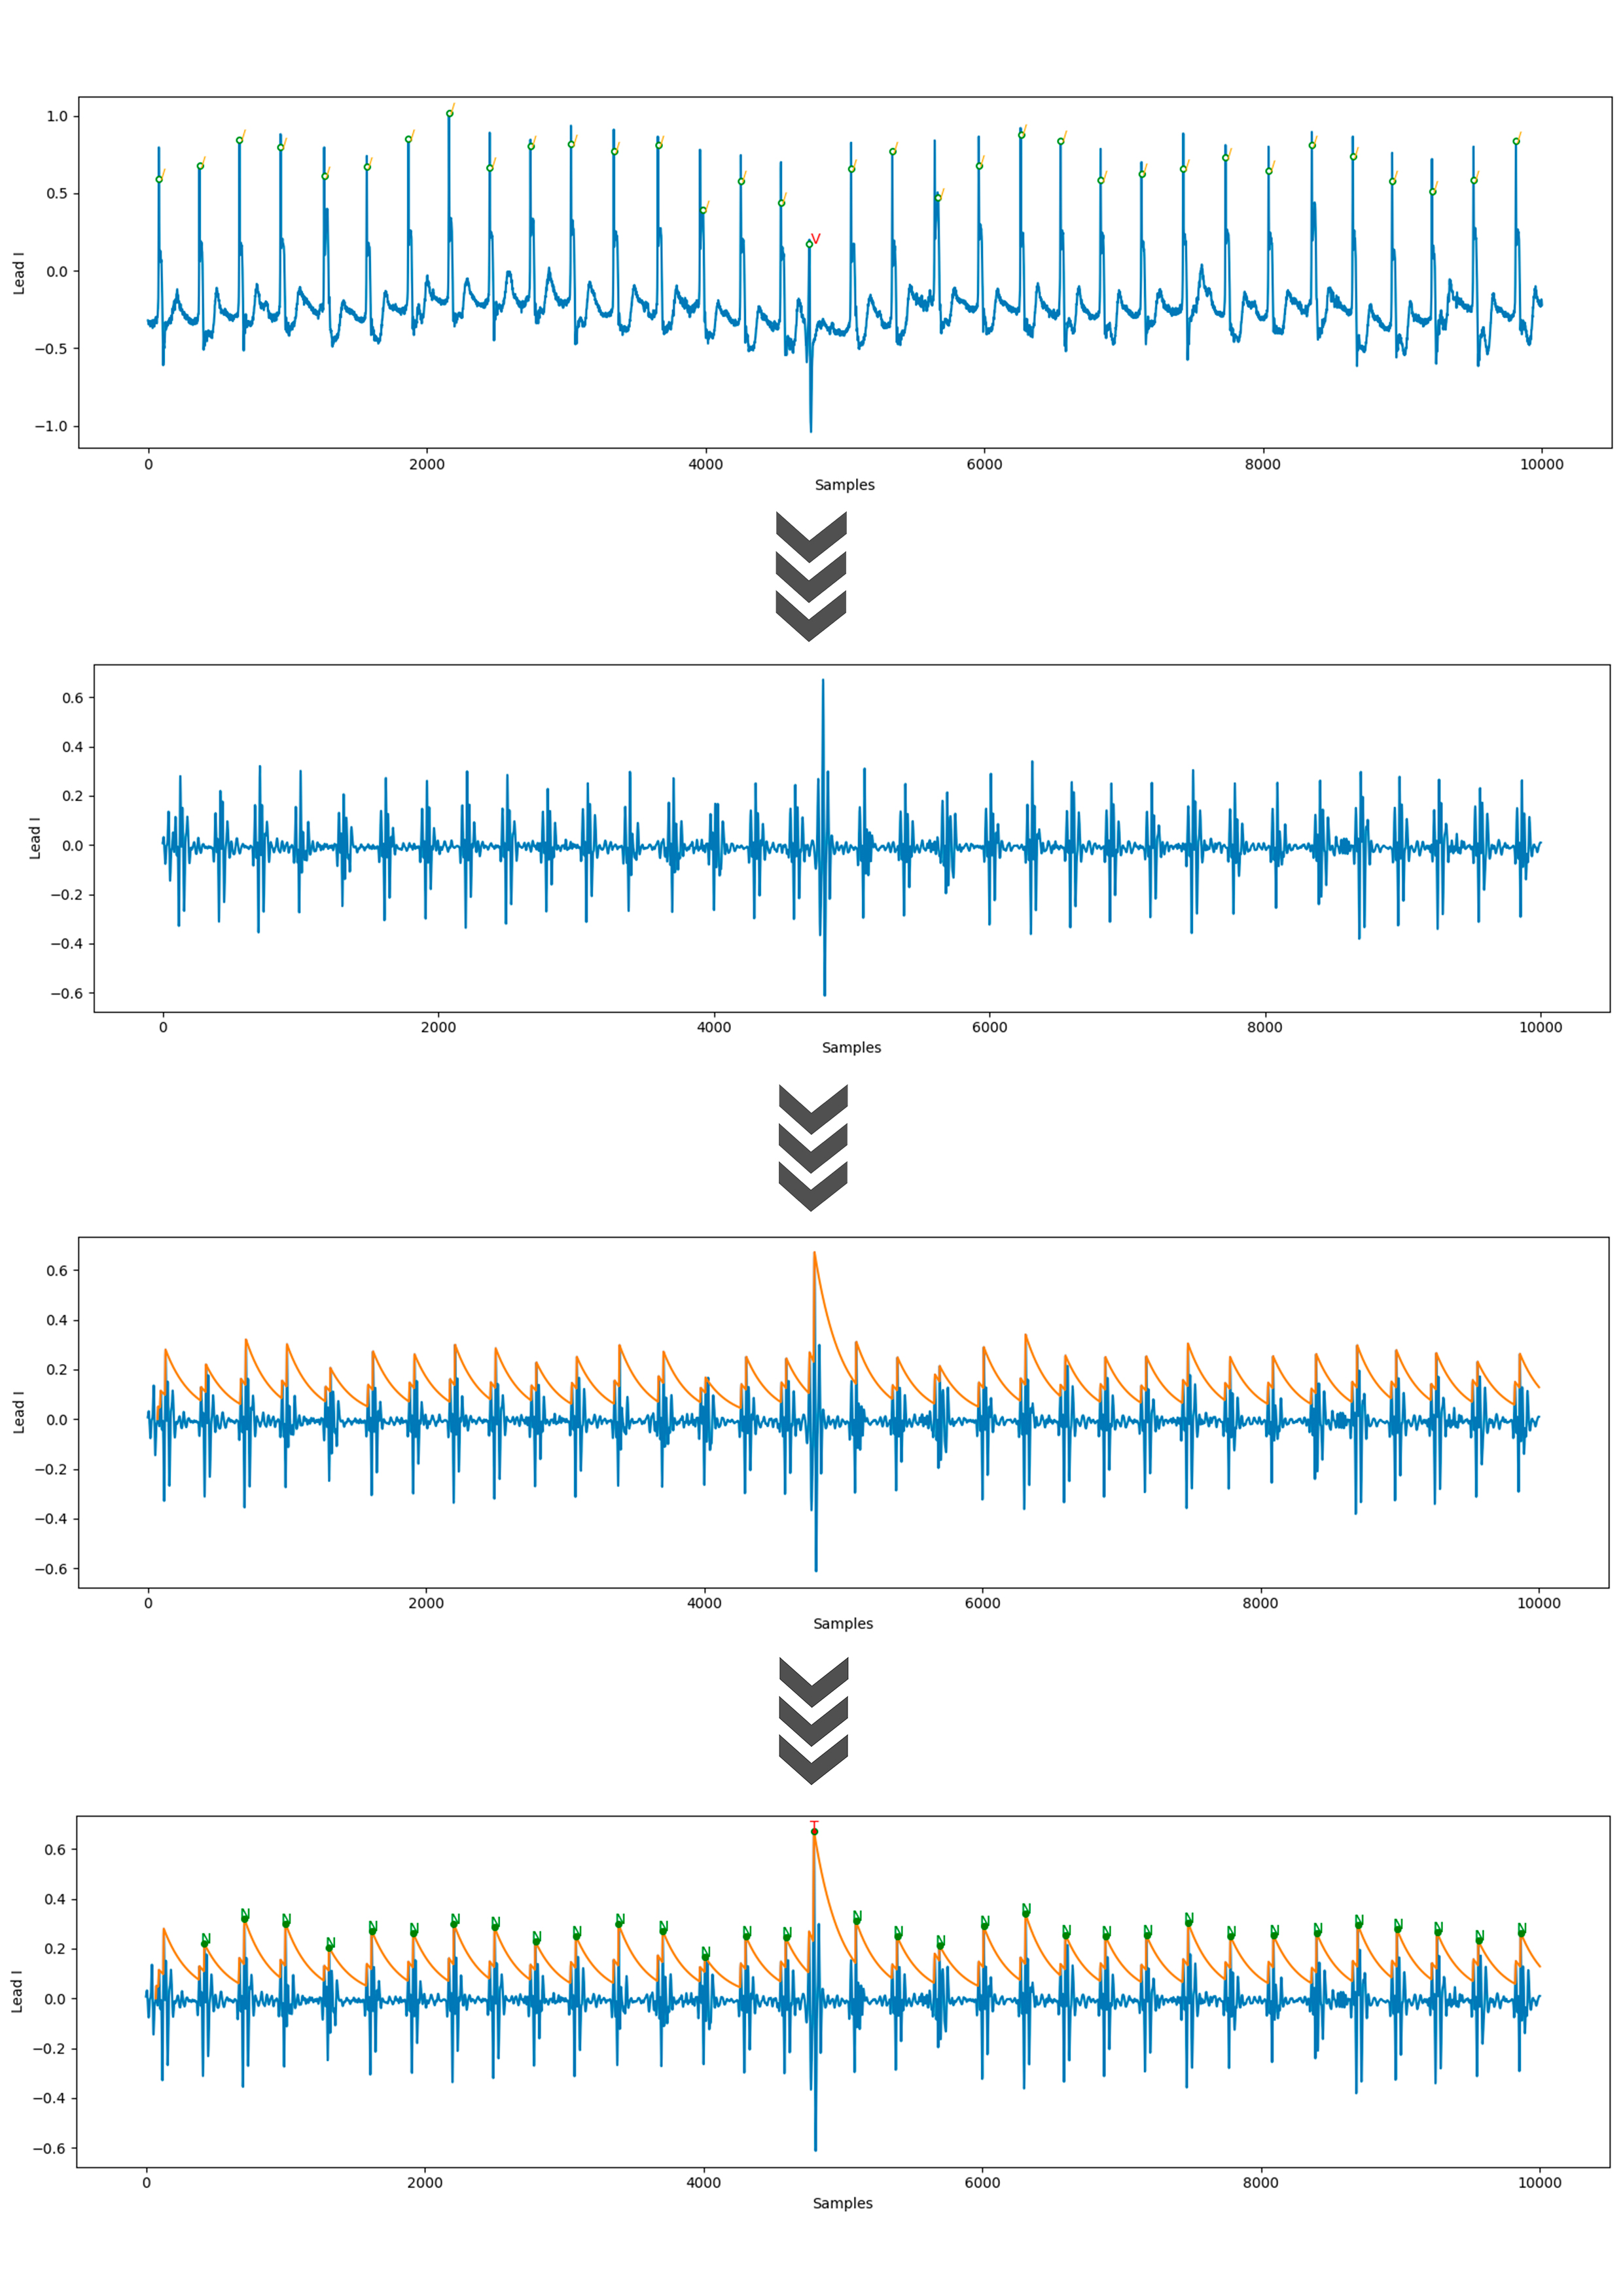
\includegraphics[width=0.7\textwidth]{./Images/img_algoritmo/esquemaGeneral.jpg}
    \caption[Representación del trascurso del prototipo]{Representación del trascurso del algoritmo durante las distintas etapas}
    \label{fig:esquemaGeneral}
\end{figure}

\section{Recopilación de los datos}
Para la recopilación de los datos se utilizará la librería \textit{wfdb} \cite{WFDB} que se encarga de proporcionar funciones para leer y escribir archivos de diferentes formatos que contienen señales biomédicas, como archivos de registro de señales (por ejemplo, formato .dat), archivos de anotaciones (por ejemplo, formato .atr) y archivos de cabecera (por ejemplo, formato .hea). 

Los pacientes vienen identificados por un identificador (por ejemplo, 101) y hay 3 ficheros por paciente, 
con extensiones .dat, .atr y .hea

Se descarga la base de datos \cite{desai2021low} con la función de la librería de \textit{wfdb}, \textit{dldatabase} que recoge 
la señal del paciente y las anotaciones de los cardiólogos sobre cada pico QRS.


\lstset{language=python, breaklines=true, basicstyle=\footnotesize}
\begin{lstlisting}[frame=single]
#download the database if not available
if os.path.isdir("mitdb"):
	print('You already have the data.')
else:
	wfdb.dl_database('mitdb', 'mitdb')
\end{lstlisting}

Los pacientes de la base de datos se han hecho una prueba de 30 minutos con una frecuencia de muestreo de 263 sps (\textit{samples per second}), lo que en la señal 
equivale a 650000 \textit{samples}.

\lstset{language=python, breaklines=true, basicstyle=\footnotesize}
\begin{lstlisting}[frame=single]
sampfrom = 0
sampto = 650000
record = wfdb.rdsamp('mitdb/102', sampfrom=sampfrom, sampto=sampto)
annotation = wfdb.rdann('mitdb/102', 'atr', sampfrom=sampfrom, sampto=sampto)
\end{lstlisting}

Por último, para visualizar esta señal con las anotaciones de los cardiólogos y poder comparar con las anotaciones que realiza el algoritmo se usará la librería \lstinline{matplotlib.pyplot} \cite{Matplotlib}. Con esto se mostrará la señal original con las anotaciones y la señal filtrada con las anotaciones del algoritmo como en \Cref{fig:102filtradoysinfiltrar}

\section{Filtrado de la señal original}
Este filtrado es llevado a cabo por el filtrado FIR. El filtrado FIR, que significa \textit{Finite Impulse Response} (respuesta finita al impulso), es un tipo de filtro utilizado en el procesamiento de señales digitales y analógicas. La fórmula que se utilizará para el filtrado es la siguiente:

\[ Y[i] = \sum_{k=0}^{N_x -1} b_k \cdot x[i-k] \]

Siendo $b$ son los coeficientes del filtrado y $x$ los valores de la señal original a filtrar.

Los coeficientes se almacenan en una lista de 99 valores en punto flotante simétricos que se iteran de forma circular, con lo que después de ejecutar el último valor vuelve de nuevo al primero.  

Para el filtrado se usa la función \lstinline{lfilter} de la librería \lstinline{scipy.signal} \cite{SciPy}.

\lstset{language=python, breaklines=true, basicstyle=\footnotesize}
\begin{lstlisting}[frame=single]
    filtered_signal = lfilter(filter_taps_99_6_28, 1.0, original_signal)
\end{lstlisting}

\section{Detección de picos QRS}

El algoritmo de detección de picos está representado en esta función que recibe la señal filtrada y trata de detectar los picos QRS.

Este algoritmo está basado en el que se usa en el documento \cite{desai2021low} donde en el 4.1.2 muestran una máquina de estados del proceso que realizan.

\begin{figure}[h!]
    \centering
    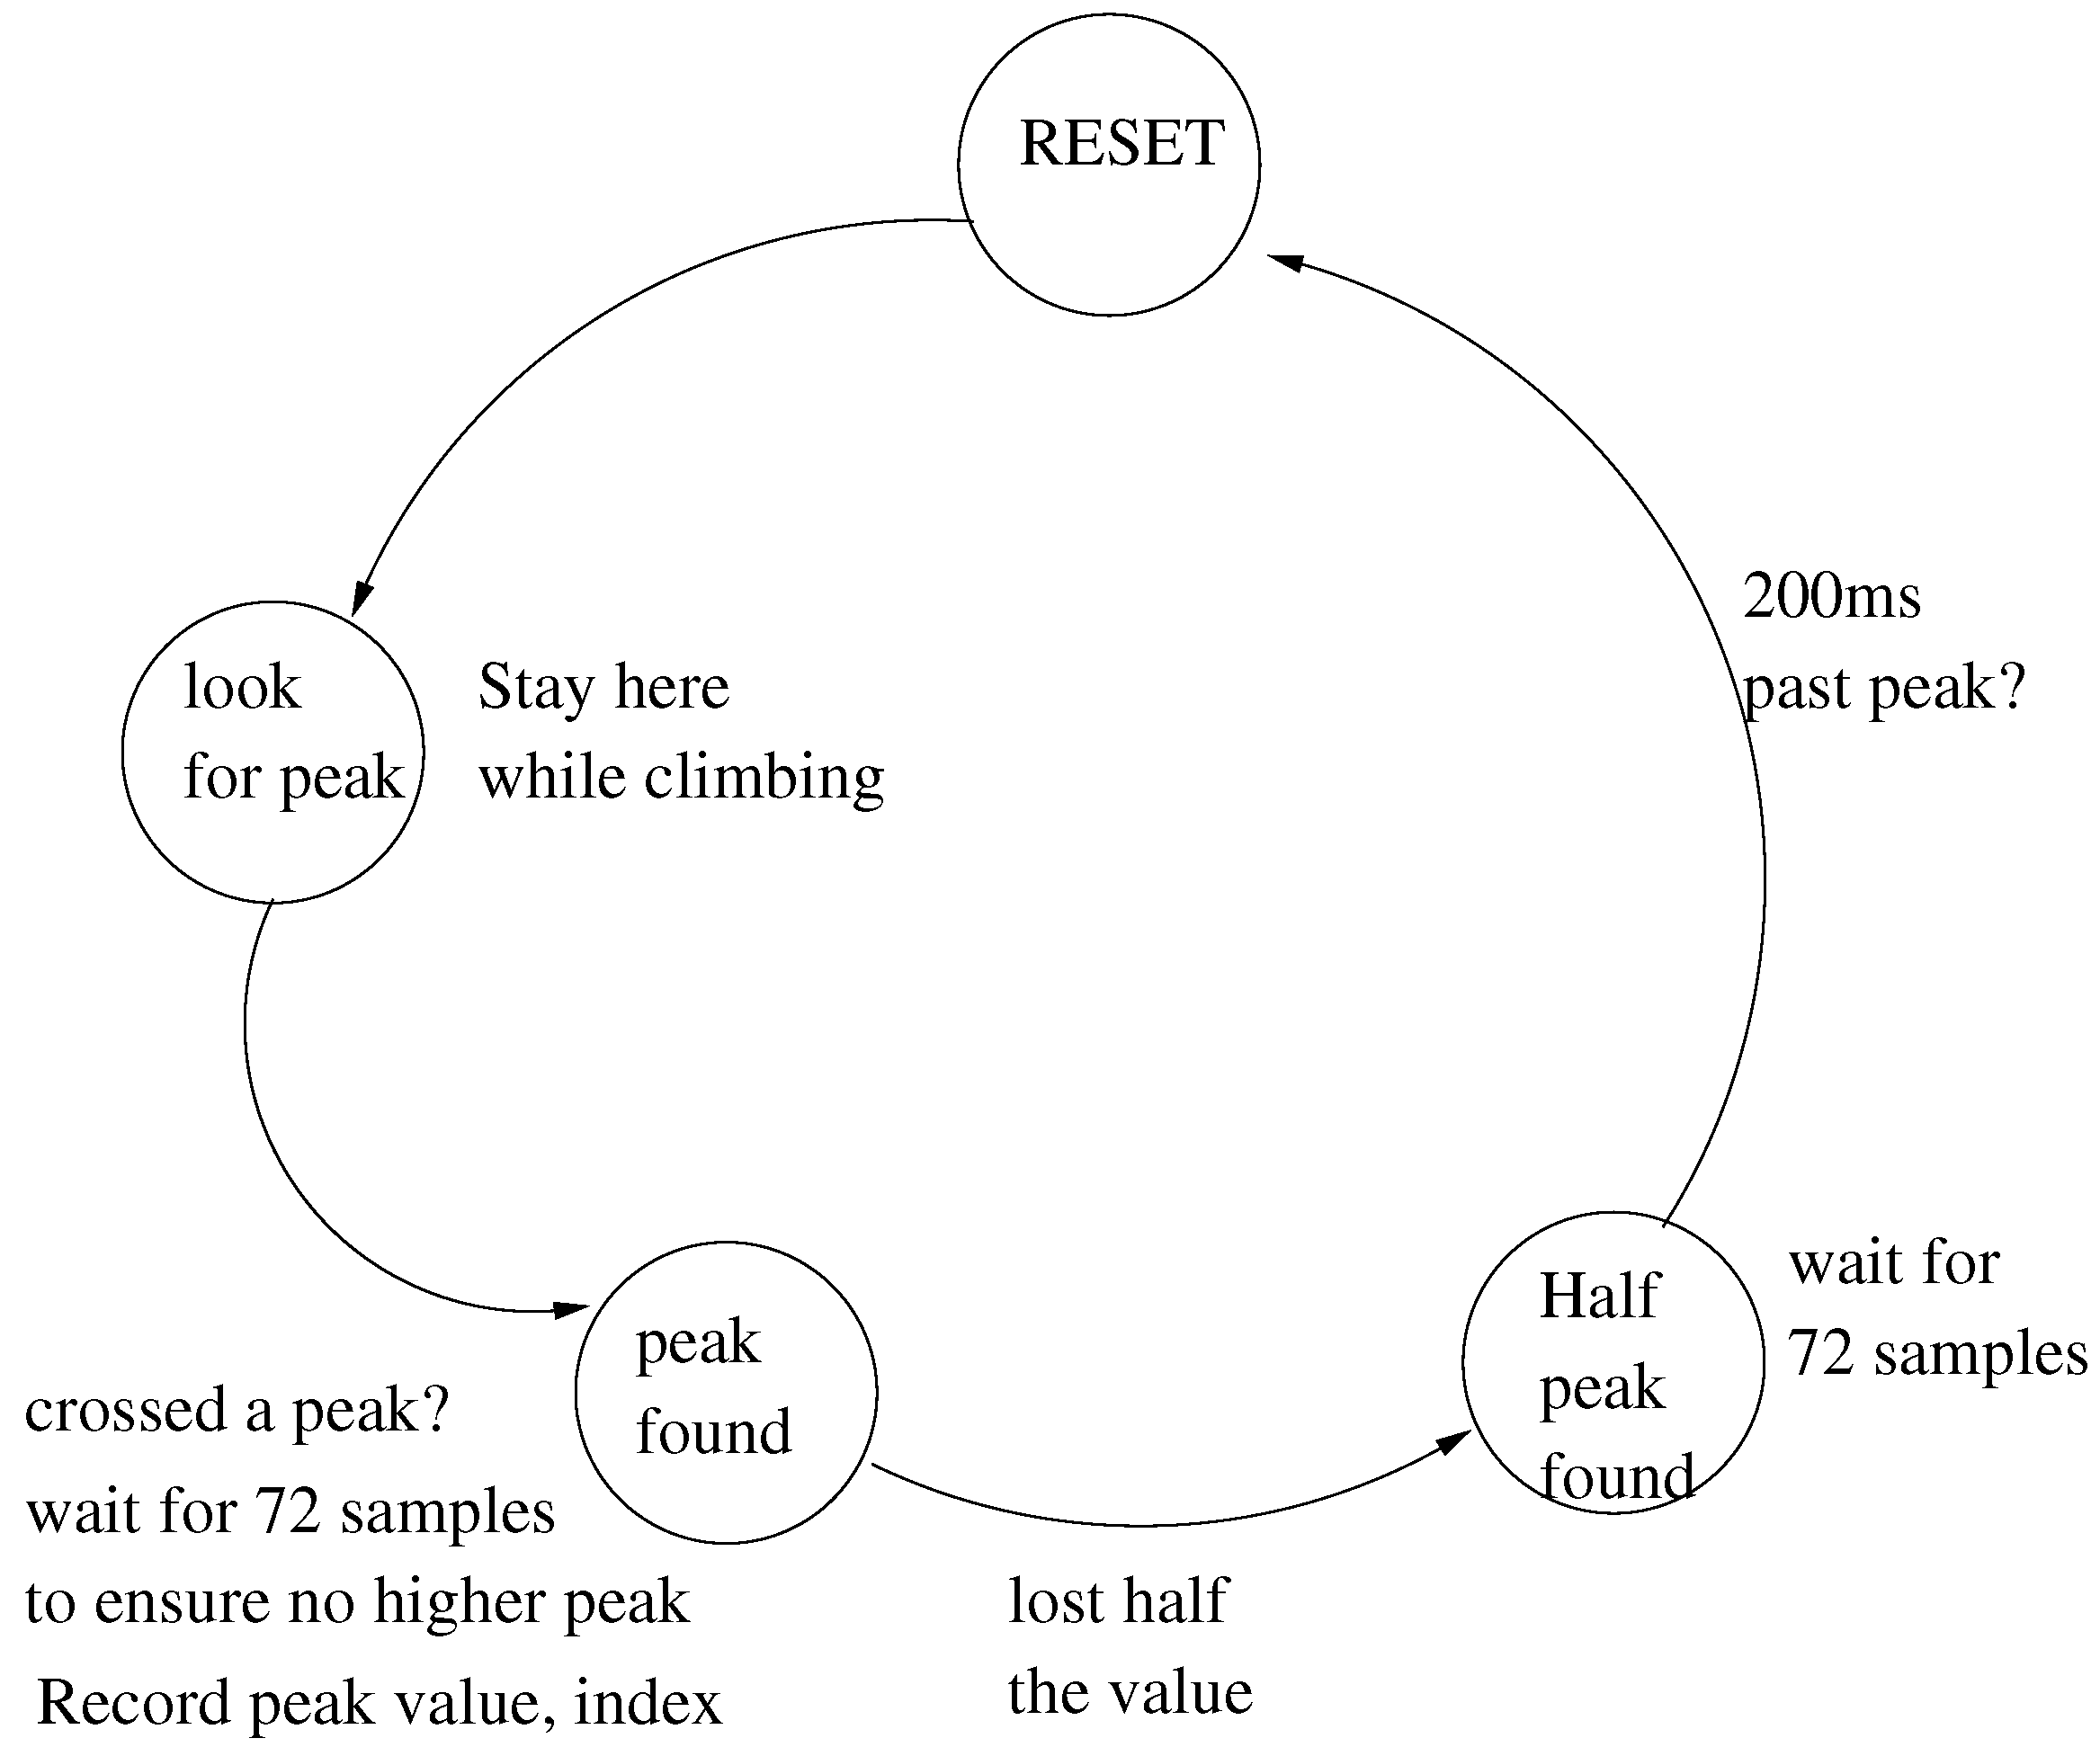
\includegraphics[width=0.6\textwidth]{./Images/img_algoritmo/fsm_mdpi.png}
    \caption{Máquina de estados de algoritmo de detección de picos de estudio de caracterización de señales usando polinomios de Hermite \cite{desai2021low}}
    \label{fig:fsm_mpdi}
\end{figure}

El algoritmo realizado es distinto a este, ya que es una versión simplificada de un algoritmo de detección de picos y no llega a ser tan funcional por la falta de un \textit{cutoff} dinámico. Esto se debe a que a veces hay una distancia entre los picos QRS superior a 72 muestras por lo que cause que en algunas ocasiones detecte el ruido como un pico QRS, ya que después de las 72 muestras no se ha encontrado una señal. Es por eso que, en un proyecto en el que se sabe que los picos QRS van a estar a distancias distintas entre sí, este algoritmo no sirve y hay que modernizarlo.

Aun así, si bien el algoritmo creado es distinto a ese, se replica el tener que esperar a 72 muestras para asegurarse de que no se encuentra un pico superior y así poder considerarlo como un pico QRS. Es por ello que definimos la variable \lstinline|samples_around_peak| como 72 para comparar dicha condición. Para hallar el pico más alto se necesita definir un pico en \lstinline{last_peak} y si se encuentra otro pico se realiza el máximo entre el pico encontrado y el de \lstinline{last_peak}.

\lstset{language=python, breaklines=true, basicstyle=\footnotesize}
\begin{lstlisting}[frame=single]
last_peak = max(last_peak,signal[i])
\end{lstlisting}
\subsection{Uso del \textit{cutoff}}
El \textit{cutoff} es un umbral bajo con el cual se ignora la señal. Solo cuando los valores de señal son mayores que el \textit{cutoff}, entra en juego la detección de pico QRS. Un \textit{cutoff} es importante pues, de lo contrario, puede que detecte falsos positivos, ya que se buscan máximos en un rango de 72 muestras y puede que se busquen máximos en un intervalo de la señal donde no hay picos QRS.

Debido a la variación de las señales entre pacientes y la variación producida por la activación del marcapasos, el uso de un \textit{cutoff} estático, como el que se representa en la \cref{fig:cutoffestatico}, se hizo inconsistente para la detección de picos, es por ello que finalmente se utilizó un \textit{cutoff} dinámico, como se puede ver en la \cref{fig:cutoffdinamico}. Este se adapta mejor a la amplitud de ondas en la señal y así no captar picos QRS de más o de menos.

El \textit{cutoff} dinámico recoge ese nombre, ya que su valor depende si se ha encontrado un pico o no, ya que cuando se encuentra un pico por encima del \textit{cutoff} anterior, el valor del \textit{cutoff} pasa a ser el del pico, por otro lado, cada vez que no se encuentre ningún pico La función del \textit{cutoff} pasa a ser la siguiente.
\[cutoff = cutoff - cutoff/(256 - 64)\]

Se han dado los valores (256 - 64) a la fórmula para que, a la hora de replicar el programa en hardware, fuese más fácil la división, ya que solo habría que desplazar los bits, Sin embargo, como al final se terminó haciendo en un módulo de división en punto flotante cualquier valor es válido para la división aunque debido al buen desempeño del valor en el programa se decidió mantener el valor.

\begin{figure}[h!]
    \centering
    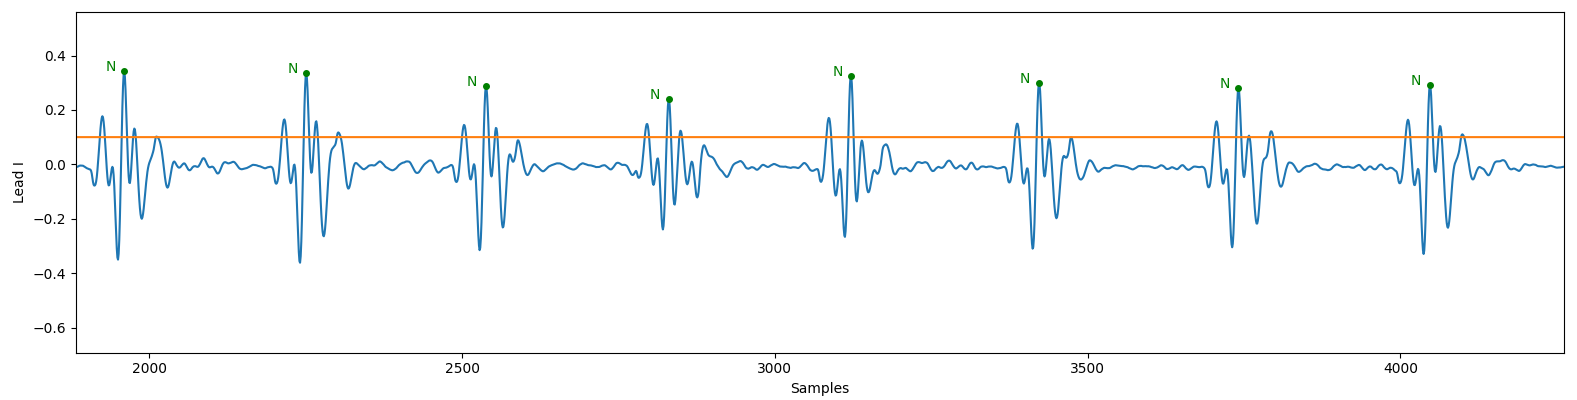
\includegraphics[width=0.9\textwidth]{./Images/img_algoritmo/cutoffestatico.png}
    \caption[Imagen de \textit{cutoff} estático]{Imagen del desempeño del algoritmo con un \textit{cutoff} estático sobre el paciente 102}
    \label{fig:cutoffestatico}
\end{figure}

\begin{figure}[h!]
    \centering
    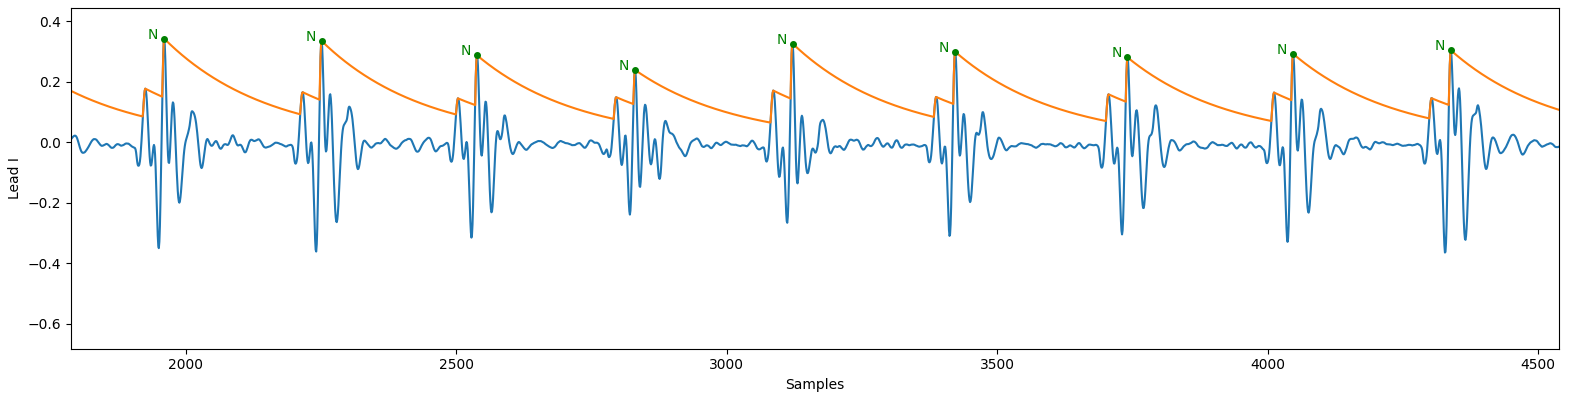
\includegraphics[width=0.9\textwidth]{./Images/img_algoritmo/cutoffdinamico.png}
    \caption[Imagen de \textit{cutoff} dinámico]{Imagen del desempeño del algoritmo con un \textit{cutoff} dinámico sobre el paciente 102}
    \label{fig:cutoffdinamico}
\end{figure}

\begin{figure}[h!]
	\centering
    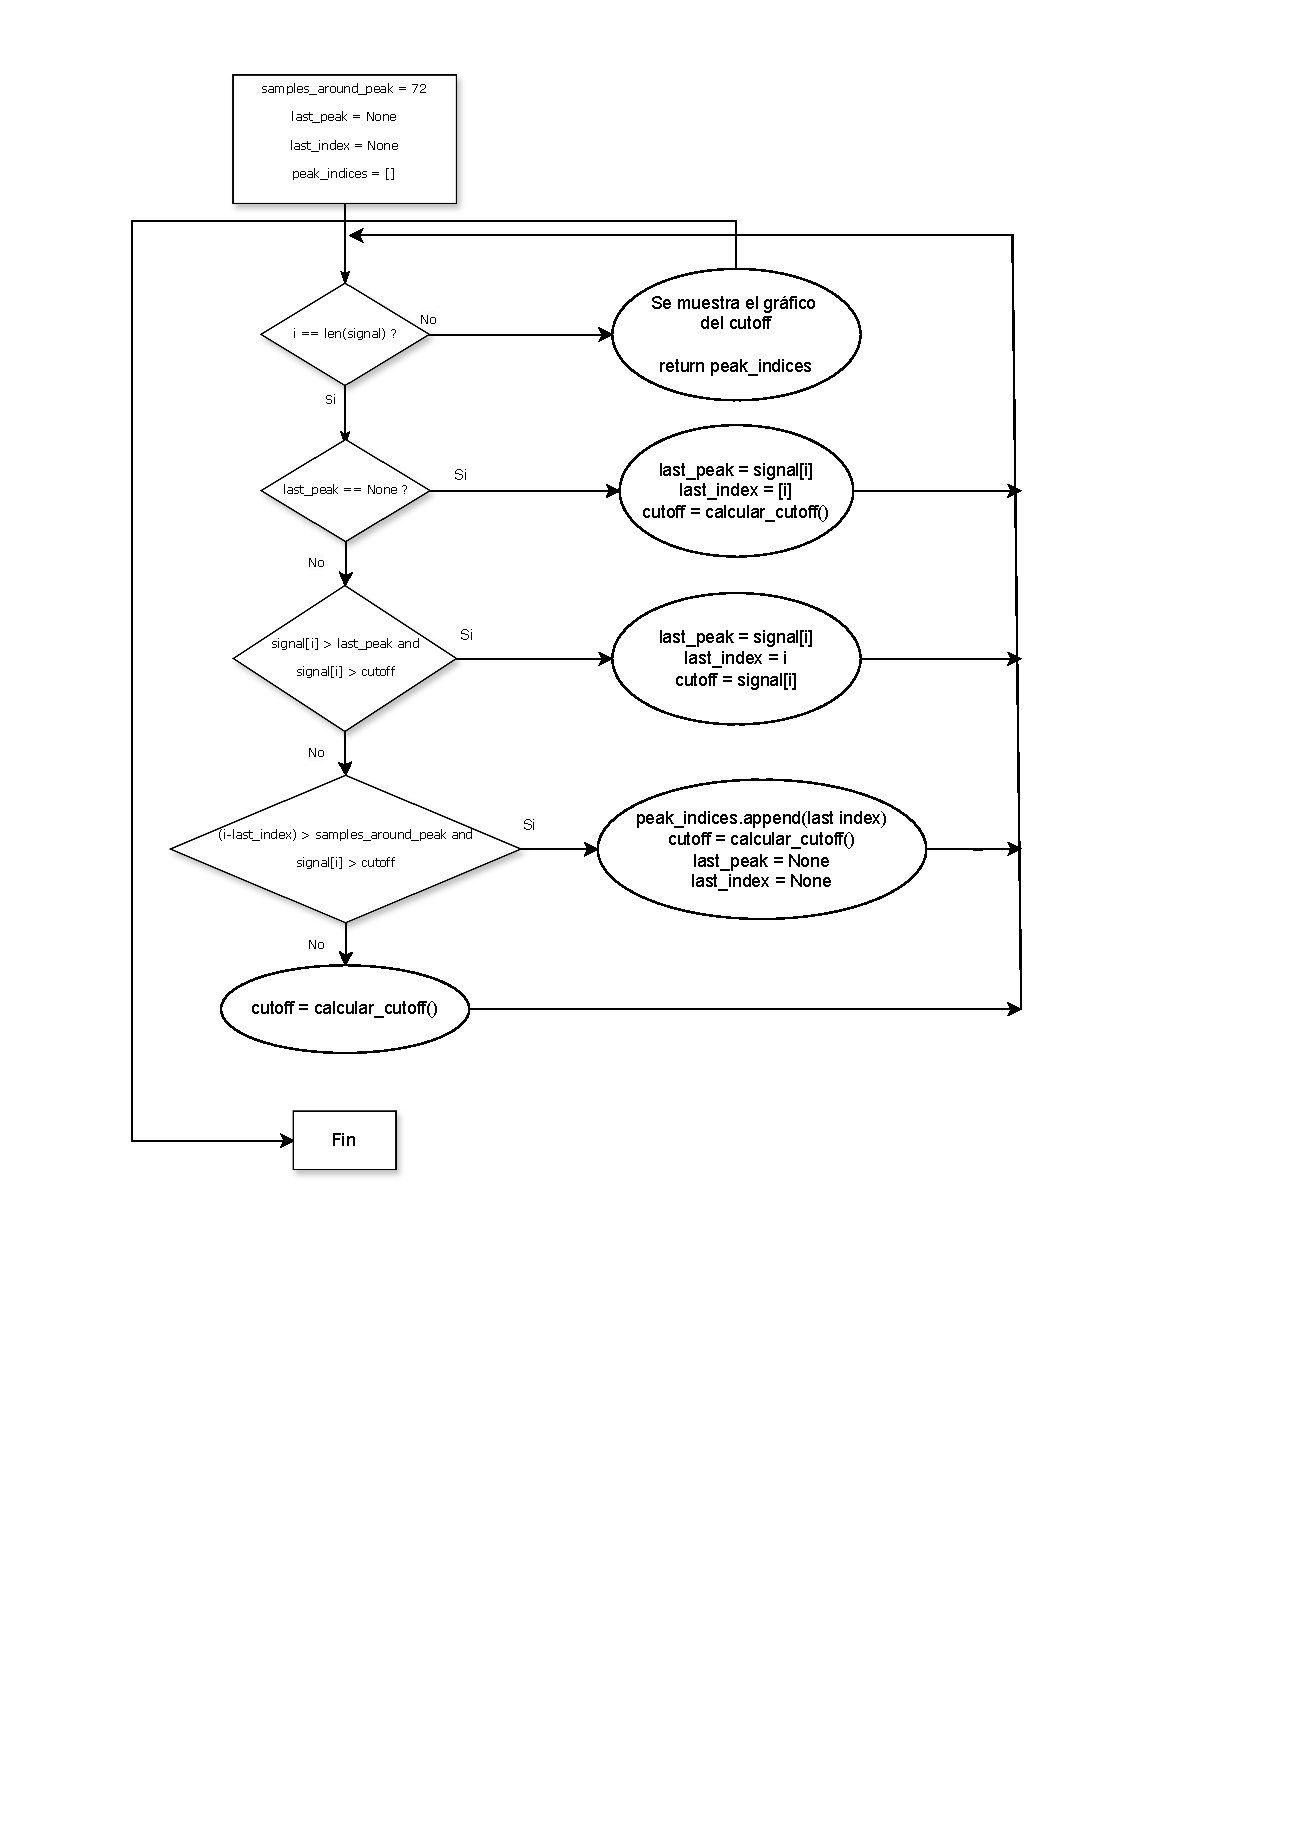
\includegraphics[width=0.99\textwidth]{./Images/img_algoritmo/Diagramapicos.pdf}
    \caption{Diagrama ASM del algoritmo de detección de picos QRS}
    \label{fig:diagramapicos}
\end{figure} 

\FloatBarrier
La salida de dicha función es un buffer de \textit{samples} que sirven como indices para indicar donde se han encontrado
los picos QRS y así poder pasar al módulo de detección de arritmias.

\section{Detección de arritmias}

El algoritmo de detección de arritmias se encarga de comprobar si se ha producido una arritmia según la
distancia entre los picos.

En la detección de arritmias es de vital importancia establecer un límite en la distancia entre los picos
para poder considerar que ha habido una arritmia o no. Esta tarea solo se pudo hacer probando con diferentes
rangos y viendo el índice de aciertos producidos en las pruebas a cada paciente de las que se hablara más adelante. 

El algoritmo va almacenando distancias entre los picos QRS (es por ello que en la primera iteración no se almacena nada)
y se declaran varias variables:

\begin{itemize}
    \item last\_distance: se utiliza para almacenar la última distancia recogida y así poder compararla con la distancia 
    actual en cálculos posteriores.
    \item counter\_buffer: utilizado para tener el valor de la posición del buffer donde se escribe.
    \item counter\_arrythmia: utilizado para indicar si la distancia anterior fue una arritmia.
    \item TNRange: Se utiliza para indicar si hay una distancia más grande de lo normal entre 2 picos QRS producido
    por una arritmia. Es importante tener esta distancia en cuenta, ya que si el ritmo del paciente vuelve a la
    normalidad se compararía la distancia entre el ritmo normal del paciente con el ritmo extendido por la arritmia,
    ya que de no tenerlo en cuenta el algoritmo lo clasificaría como arritmia como se puede ver en la \cref{fig:senial_explicacion_TNRANGE}, por ello se compara con un valor anterior
    que sea el ritmo normal del paciente.
\end{itemize}

\begin{figure}[h!]
    \centering
    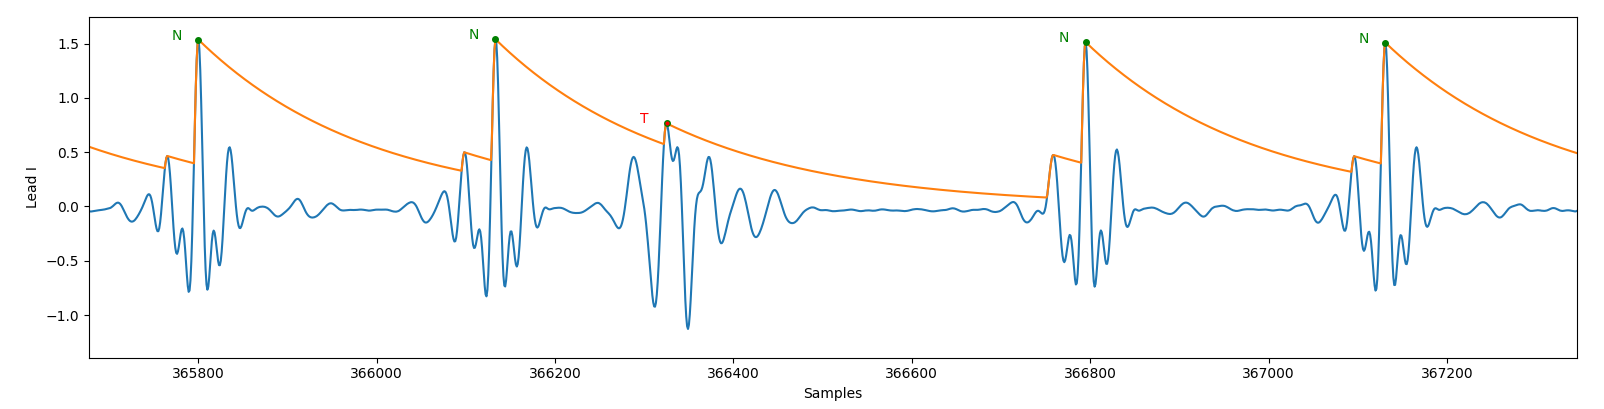
\includegraphics[width=0.9\textwidth]{./Images/img_algoritmo/senial_explicacion_TNRANGE.png}
    \caption{Cuando se detecta una arritmia, a veces, la siguiente distancia es considerablemente más grande de lo normal. Para no detectar falsos positivos, se omite esa distancia.}
    \label{fig:senial_explicacion_TNRANGE}
\end{figure}

Por ello si se ha detectado una arritmia, la siguiente distancia se compara con
la tercera última distancia escrita en el buffer que posiblemente sea una distancia causada por un ritmo normal. 
Si no se da el caso, se compara con last\_distance.

La función que compara las distancias devuelve un carácter que va a ser el que se vaya a mostrar en la gráfica. 
Si el carácter es ``N'' significa que se ha detectado un ritmo normal y por tanto solo se muestra. Sin embargo, si el 
resultado es ``T'' significa que la distancia es más corta de lo normal, se detecta la arritmia y se ponen
counter\_arritmia a 1 para saber que la distancia es más corta y TNRange a true para que el algoritmo sepa 
que la distancia que venga después puede ser una ampliada. 

\begin{figure}[h!]
	\centering
    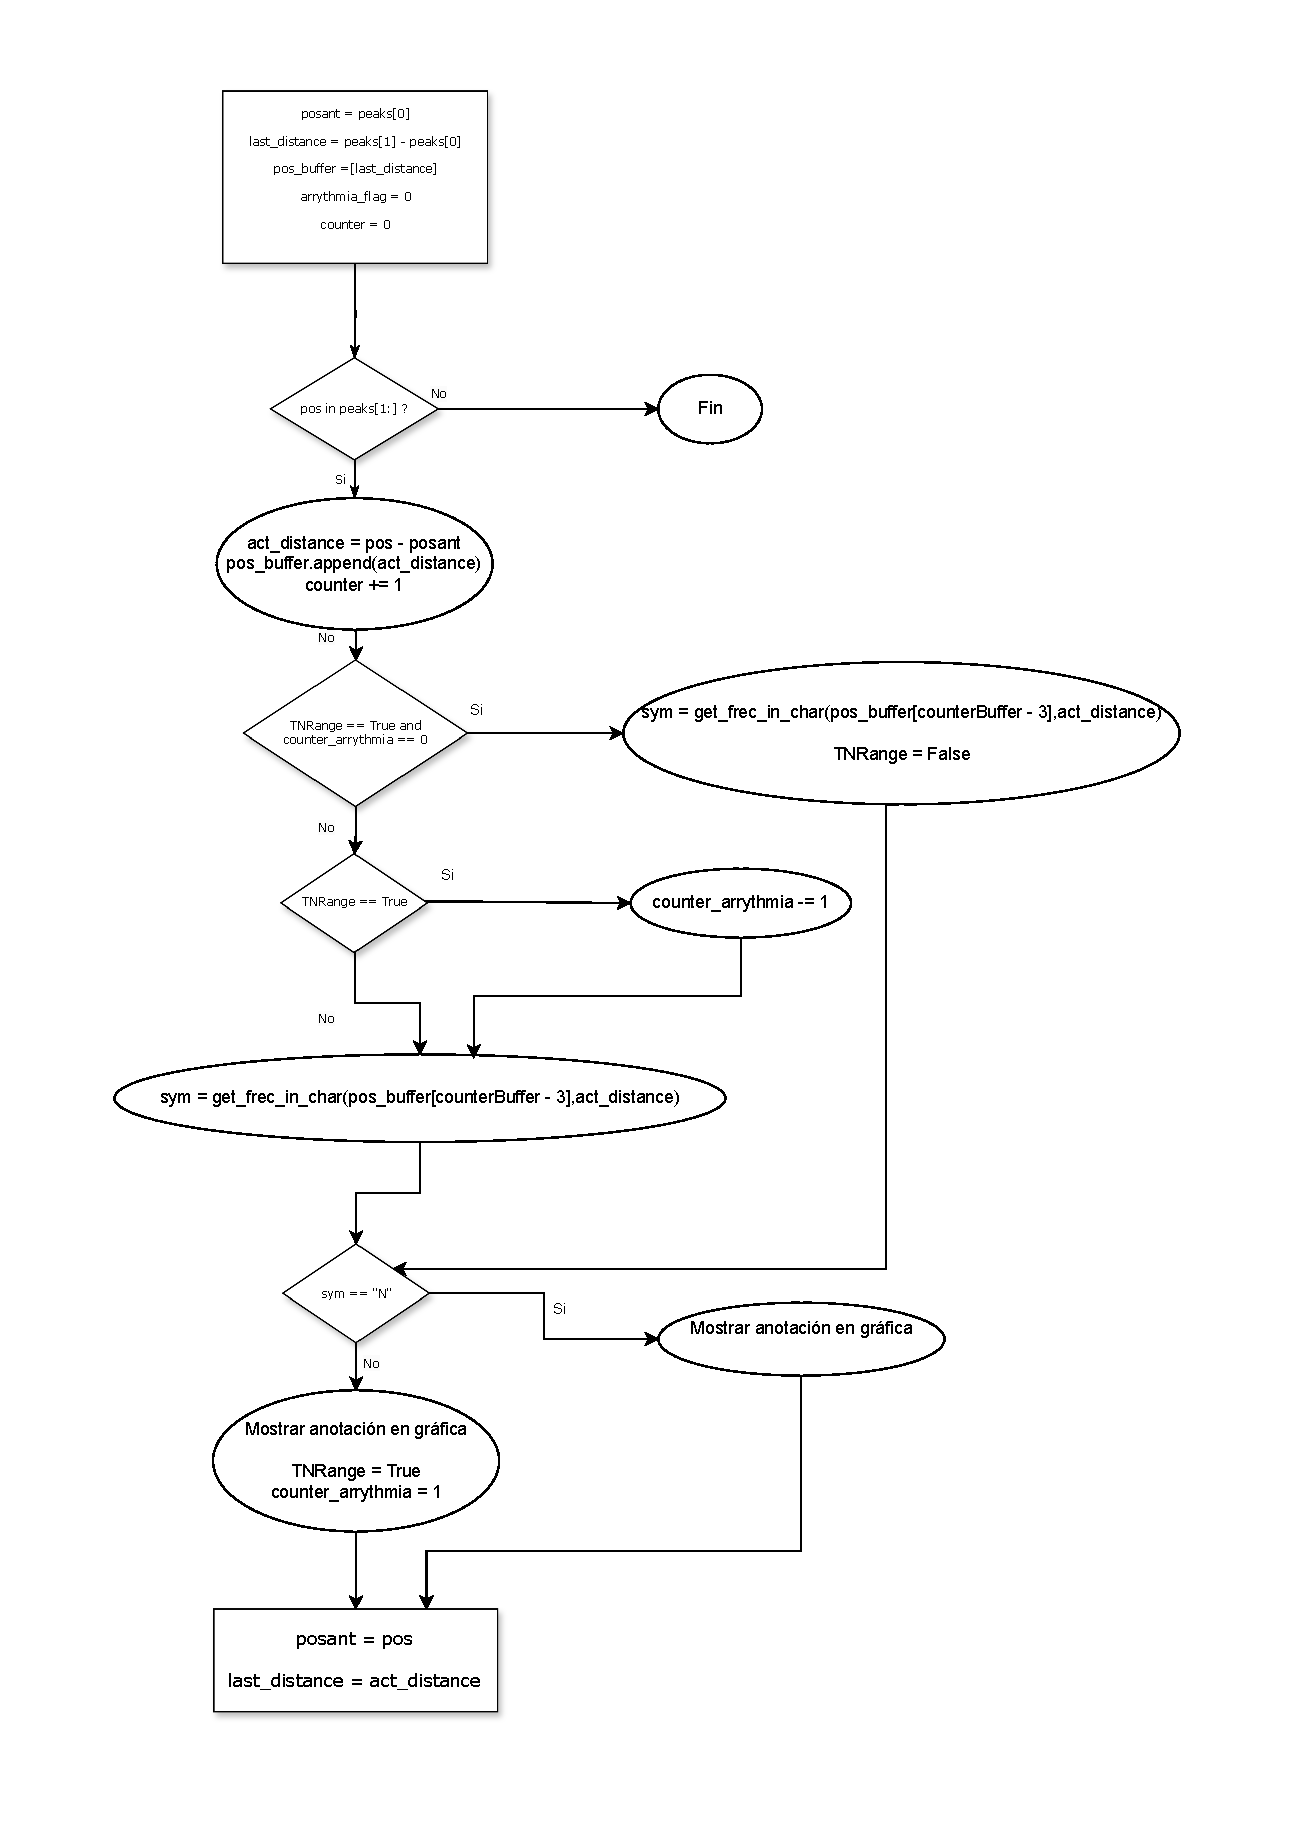
\includegraphics[width=0.9\textwidth]{./Images/img_algoritmo/Diagramaarritmias.pdf}
    \caption{Diagrama ASM del algoritmo de detección de arritmias}
    \label{fig:diagramaarritmias}
\end{figure} 

\FloatBarrier

La función \lstinline{get_frecuency_in_char()} se encarga de calcular las distancias entre el ritmo actual y un ritmo normal. 
Para ello recibe como entrada ambas distancias.

Para empezar se calcula el gap que es simplemente la diferencia que tiene la distancia anterior con la actual.

\[gap = last\_distance - actual\_distance\]

Acto seguido, se calcula el porcentaje de la diferencia de distancia con la distancia anterior que se sabe que va a ser 
un ritmo normal.

\[percentaje = (gap / last\_distance) * 100\]

Si ese porcentaje es mayor que el 15\% entonces se considera que la distancia normal es mucho mayor que la actual
y por tanto como la distancia actual entre 2 picos es pequeña, se da por hecho que hay una arritmia.

Nótese que no se le da importancia si el gap da como resultado un número negativo de cualquier tamaño, esto se debe
a que este proyecto solo está pensado para detectar contracciones prematuras del corazón, por ende solo necesitamos 
saber si la distancia actual es menor que la anterior. Además, ningún paciente parece padecer ninguna arritmia de otro
tipo.

\section{Pruebas con el algoritmo}

Se han realizado una serie de pruebas para probar el algoritmo para comprobar si las posiciones donde
se ha detectado un pico QRS coinciden con las posiciones de los picos detectados por los cardiólogos, y además se 
encargan de comparar las anotaciones de los cardiólogos con las generadas por el algoritmo.

Con dichas estadísticas es posible comparar el porcentaje de aciertos, en los que se comprende el número de 
falsos positivos (referido a los ritmos normales que el algoritmo considera arritmias) y 
falsos negativos (referido a las arritmias que el algoritmo considera un ritmo normal).

Para desarrollar estas pruebas, se ha creado una clase Pair que contenga, por cada iteración del algoritmo de detección de arritmias, el carácter que indica si el algoritmo ha detectado una arritmia o no y la posición del pico QRS analizado. Dicho objeto se inserta en una lista de Pair para luego poder comparar con las anotaciones de la señal original.

Una vez se rellena todo el buffer de Pair, se comprueban 2 cosas.
\begin{enumerate}
	\item Si se ha detectado un pico QRS en la señal filtrada y se
     corresponde con el pico de la señal original situado en un \textit{sample} de una posición aproximada.
	\item Si en el caso de que se haya detectado el pico, las anotaciones de los cardiólogos coinciden
     con las generadas por el algoritmo.
\end{enumerate} 

Para este proyecto, solo se valora si el paciente tiene un ritmo normal o una arritmia, pero las anotaciones que contiene la señal original pueden simbolizar otros problemas como la entrada del marcapasos u otros problemas con la onda T.
En la clase \textit{Annotation} de la librería \textit{wfdb} \cite{WFDB}, vienen explicadas todas las posibles anotaciones que puede haber como se muestra debajo.
\newpage
\lstset{language=python, breaklines=true, basicstyle=\footnotesize}
\begin{lstlisting}[frame=single]
    ann_labels = [
        AnnotationLabel(0, " ", 'NOTANN', 'Not an actual annotation'),
        AnnotationLabel(1, "N", 'NORMAL', 'Normal beat'),
        AnnotationLabel(2, "L", 'LBBB', 'Left bundle branch block beat'),
        AnnotationLabel(3, "R", 'RBBB', 'Right bundle branch block beat'),
        AnnotationLabel(4, "a", 'ABERR', 'Aberrated atrial premature beat'),
        AnnotationLabel(5, "V", 'PVC', 'Premature ventricular contraction'),
        AnnotationLabel(6, "F", 'FUSION', 'Fusion of ventricular and normal beat'),
        AnnotationLabel(7, "J", 'NPC', 'Nodal (junctional) premature beat'),
        AnnotationLabel(8, "A", 'APC', 'Atrial premature contraction'),
        ...
        AnnotationLabel(12, "/", 'PACE', 'Paced beat'),
        AnnotationLabel(13, "Q", 'UNKNOWN', 'Unclassifiable beat'),
        AnnotationLabel(14, "~", 'NOISE', 'Signal quality change'),
        AnnotationLabel(16, "|", 'ARFCT',  'Isolated QRS-like artifact'),
        ...
        AnnotationLabel(38, "f", 'PFUS',  'Fusion of paced and normal beat'),
        ...
    ]
\end{lstlisting}

Por ello en este proyecto solo se prestará atención a la anotación A y a la anotación V que simbolizan 
las contracciones prematuras de la aurícula y el ventrículo, las demás anotaciones sobre el pico QRS serán 
consideradas como ritmos normales.

Para comparar los picos de ambas listas, se examina el sample en el que se encuentra dicho pico en la señal original. Como los picos de la señal filtrada presentan un desfase de 50 samples respecto a la señal original, simplemente hay que comprobar si hay un pico QRS 50 samples más adelante en la señal filtrada. Adicionalmente, para evitar problemas por el filtrado de la señal, se ha establecido un margen de error de 20 samples para incluir los picos que puedan haberse desfasado debido al filtrado. Si por otro lado, el pico no se ha detectado donde tendría que haber un pico QRS puesto en la señal original, 
se pone doble guión para simbolizarlo. 

Se realiza un conteo de las anotaciones correctas en total, las anotaciones incorrectas en total, las anotaciones
correctas solo de los picos detectados como arritmia, las incorrectas de ese mismo tipo, y los picos no registrados, 
como se ve en la \Cref{fig:estadisticassacadastabla}. Todas las pruebas posteriores han sido realizadas sobre la señal del paciente 102 de principio a fin.

\begin{figure}[h!]
	\centering
    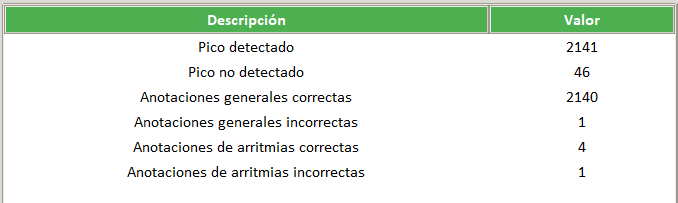
\includegraphics[width=0.69\textwidth]{./Images/img_algoritmo/estadisticassacadastabla.png}
    \caption{Métricas de detección de arritmias}
    \label{fig:estadisticassacadastabla}
\end{figure} 
\newpage

Con las estadísticas anteriores se pueden hallar los picos totales que tiene la señal original, el porcentaje de picos 
detectados, el porcentaje de picos no detectados, el porcentaje de arritmias detectadas 
correctamente. Esto está representado en la \Cref{fig:estadisticasporcentaje}.

\begin{figure}[h!]
	\centering
    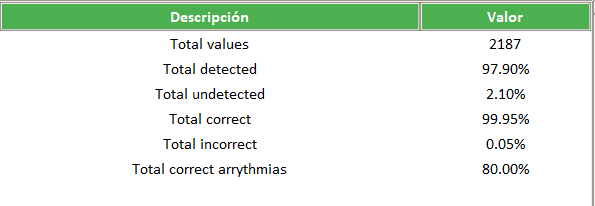
\includegraphics[width=0.9\textwidth]{./Images/img_algoritmo/estadisticasporcentaje.png}
    \caption{Porcentajes de detección de arritmias}
    \label{fig:estadisticasporcentaje}
\end{figure} 

Adicionalmente se puede sacar una matríz de confusión como en la \Cref{fig:matrizdeconfusion}, donde se establece como verdadero la aparición de arritmias en la señal original y como positivo a la detección de arritmias sobre la señal procesada por el algoritmo. En el caso del paciente 102, no ha habido arritmias en 2136 picos, ha habido 4 arritmias detectadas correctamente y un falso positivo que indica que el algoritmo ha detectado una arritmia, pero no era.

\begin{figure}[h!]
	\centering
    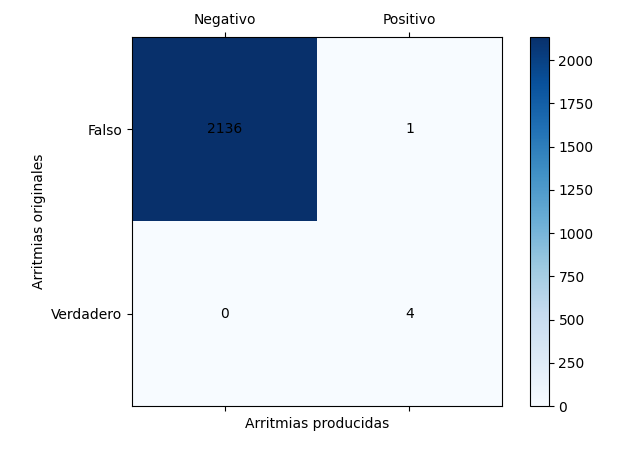
\includegraphics[width=0.9\textwidth]{./Images/img_algoritmo/matrizdeconfusion.png}
    \caption[Matríz de confusión]{Matríz de confusión del funcionamiento del algoritmo sobre la señal del paciente 102}
    \label{fig:matrizdeconfusion}
\end{figure} 

Dichas pruebas mostradas se aplican solo para un paciente, pero es posible aplicar estas pruebas a todos los pacientes.
Para ello se ha creado un nuevo programa de \textit{python} que se encarga de realizar la misma prueba para los pacientes cuyo id está
almacenado en un buffer.

Este programa tiene 2 modos, uno procesa un paciente individualmente y el otro itera sobre una lista con los identificadores de los pacientes para procesarlos a todos. La lógica del algoritmo visto anteriormente está contenida en una nueva función llamada \lstinline{calculations()}.

Las pruebas que se realizan para este algoritmo son iguales que en el programa anterior, pero también
se han realizado las siguientes estadísticas.

\begin{enumerate}
	\item La media de los picos detectados de cada paciente.
	\item La media de las arritmias correctas detectadas en cada paciente.
\end{enumerate} 